\documentclass[letterpaper,onecolumn,titlepage]{Ythesis}

\usepackage{graphicx}
\graphicspath{{sections/figs/}{.figs/}}

\usepackage[backend=bibtex, style=numeric-comp]{biblatex}
\bibliography{main}

\usepackage{array,multirow,graphicx}
\usepackage{subfiles}
\usepackage{url}
\usepackage{amsmath}



\title{Visualizing Conditional Dependencies}
\author{Hannah Aizenman}
\committee{Dr. Michael Grossberg(Advisor), Dr. Robert Haralick, Dr. Lev Manovich, Dr. Huy Vo}
\submitted{}
\abstract{Many datasets are too large or complex to discern patterns simply through visualizing the observations in them, so researchers instead compute the distributions of select variables and explore under what conditions they occur. While there are many visualization techniques that preserve variable type, dimensionality, and mutlivariate relationships, the complexity increases when also trying to illustrate distributions and conditional relationships. This survey presents a sampling of techniques for visualizing distributions and densities conditioned on variables that are categorical or quantitative, discrete or continuous, and potentially have or infer dimensional dependencies. 
}
\begin{document}
\makefrontmatter

\section{Introduction}
\label{sec:introduction}

\begin{figure}
  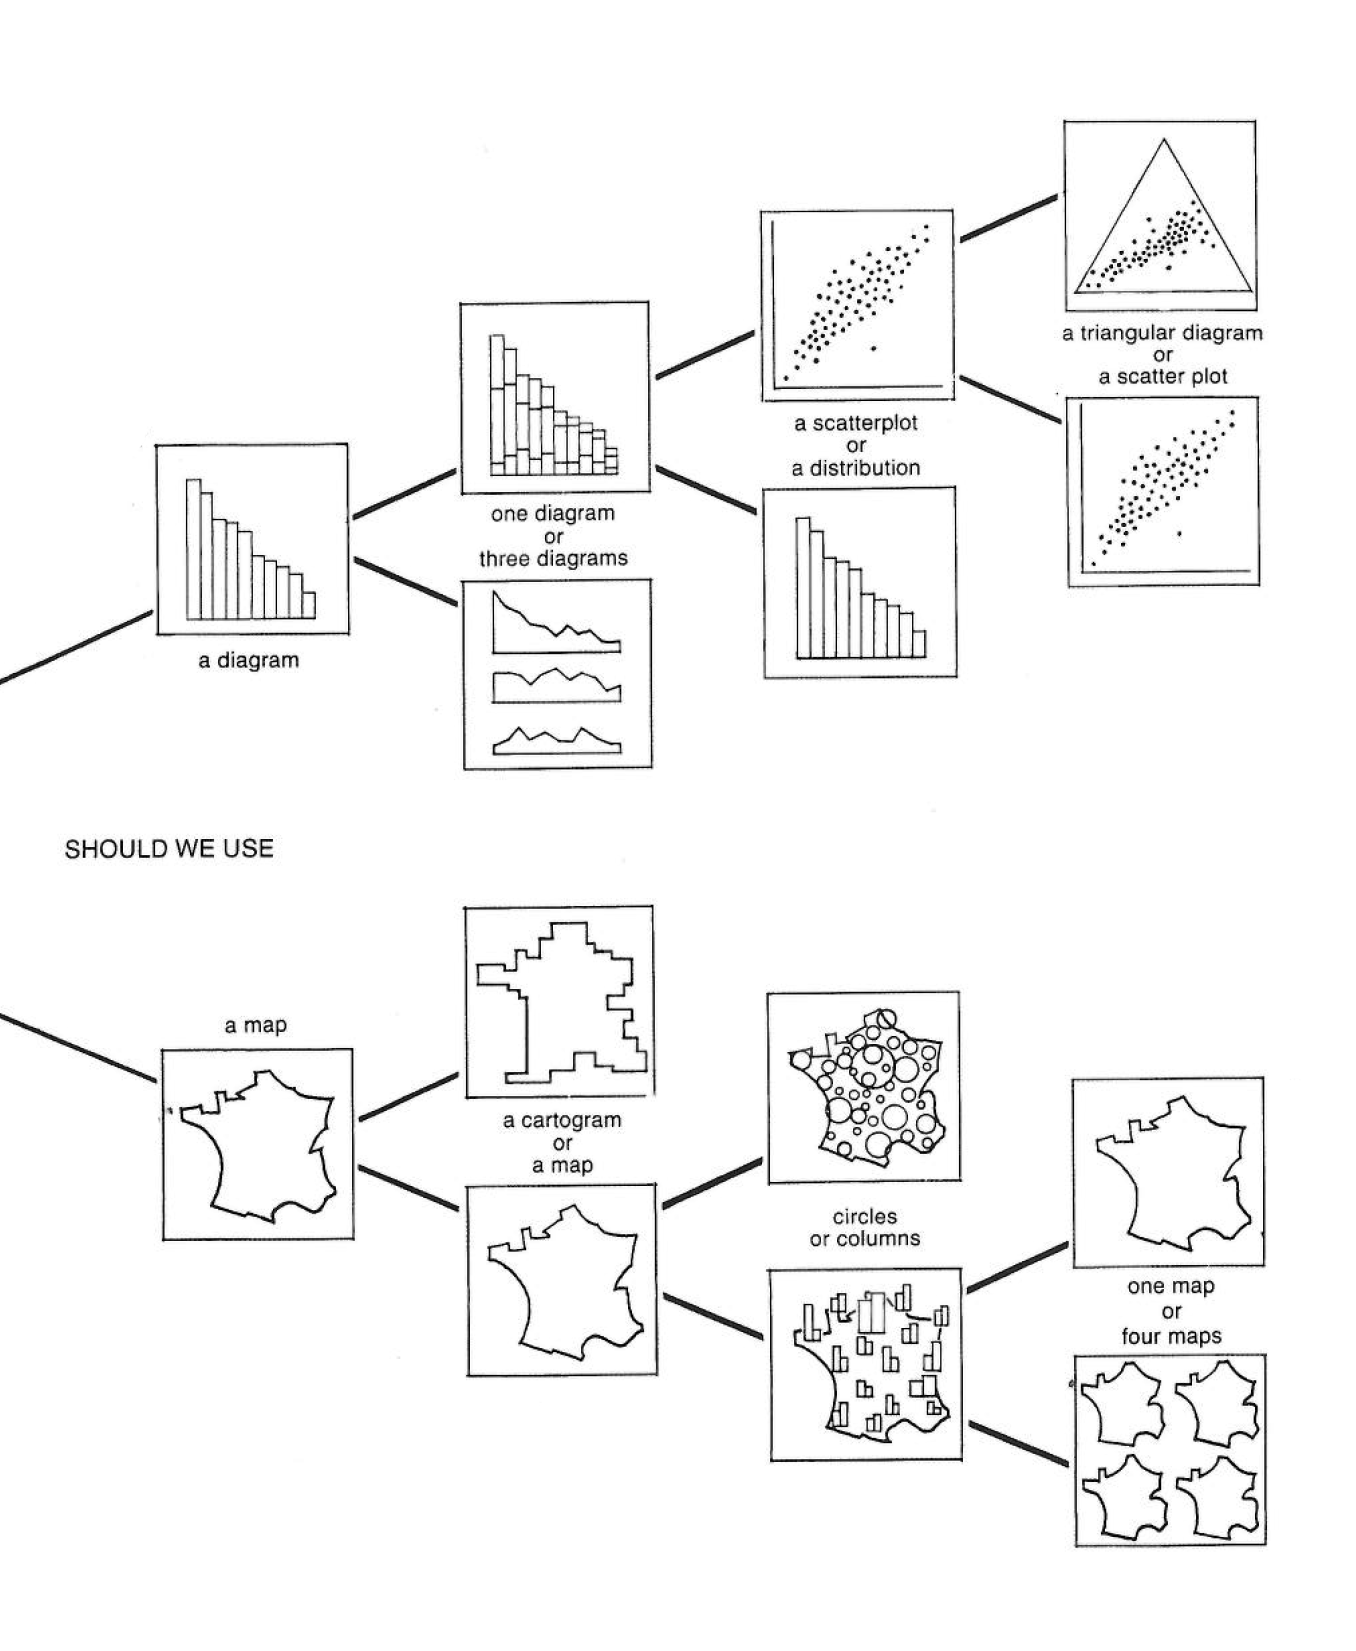
\includegraphics[width=\textwidth]{chart_chooser.png}
  \caption{From Bertin's Semiology of Graphics \cite{bertin_semiology_2011}, this diagram illustrates various ways of representing information about the French workforce in 1954.}
  \label{fig:chart_chooser}
\end{figure}

In Semiology of Graphics, Bertin \cite{bertin_semiology_2011} presents a dataset of the French work force in 1954. This dataset aggregates the workers by region and by sector, and so is structured as follows:
\begin{itemize}
	\item department (geographic region of France)
	\item  number of employees per thousands in each sector
		\begin{itemize}
			\item primary: agriculture
			\item secondary: industry 
			\item tertiary: commerce, transportation, services
		\end{itemize}
\end{itemize}

In figure~\ref{fig:chart_chooser}, Bertin explores some potential visualizations of the data, and in doing so also illustrates the trade-offs these visualizations make. The first bar graph in the tree shows the number of works per sector, but discards the categorical and encodes the spatial as each bar. Categories can be included using a stacked bar chart or three independent bar charts; the former  better preserves the proportionality between sectors within each region, while the latter better displays the regional distribution within each sector. Discarding the geographic attributes allows even more interrogation of the relationships within and between categories, via histograms and scatter plots respectively. 

While some of these approaches include the department as a the y variable, to some extent they discard the geographic information encoded in the department because this data has a physical counterpart that is not referenced in the visualization. To explicitly show this geographic information, Bertin proposes a second branch of map based visualizations. Taking the same sort of path as the upper branch, Bertin first proposes a map of how the entire workforce is distributed spatially over France. He then suggests a cartogram to show relative differences between geographic regions. As in the upper branch, he then incorporates the sector information; he proposes bubble charts and bar charts to highlight inter-sector differences and disaggregates the sectors and visualizes them as different maps to show how each sector is distributed over France. I

In these visualizations, not only is Bertin showing how many people are in the French workforce in 1954, but he is also showing how that number is conditionally dependent on categorical information such as sector and department. With respect to department, he also tries to preserve the geographic distribution of the data. Figure~\ref{fig:chart_chooser} is mostly showing the number of employees given department, category, or both. While disaggregating employees over sector and geography provides a rich set of potential factors in employee count, it is also somewhat difficult to visualize if the goal is to preserve both regional and categorical differences. While 4 maps is a small enough number to not be overwhelming, they forewarn that this technique would likely not work for a larger number of sectors. 


Despite ostensibly being a categorical variable, department can also be a dimension \cite{munzner_what:_2014} on which either number of employees or sector can depend since it maps to physical space rather than a measurement. Number of employees and the sector are traditional quantitative and categorical measurement types. This distinction of variable type serves as a basis for understanding what conditional dependencies are explored within each visualization:

% Please add the following required packages to your document preamble:
% \usepackage{mcr}
% \usepackage{graphicx}


\let\mcn\multicolumn
\let\mcr\multirow

\begin{table}[]
\centering
\resizebox{\textwidth}{!}{%
\begin{tabular}{ccl|l|l|l|l|}
\cline{4-7}
\mcn{1}{l}{}                                  & \mcn{1}{l}{}                              &       & \mcn{4}{c|}{Probability of}                                             \\ \cline{4-7} 
\mcn{1}{l}{}                                  & \mcn{1}{l}{}                              &       & \mcn{2}{c|}{Independent} & \mcn{2}{c|}{Dependent (Dimensional)} \\ \cline{4-7} 
\mcn{1}{l}{}                                  & \mcn{1}{l}{}                              &       & Categorical     & Quantative     & Categorical   & Quantative           \\ \hline
\mcn{1}{|c|}{\mcr{4}{*}{Conditioned On}} & \mcn{1}{c|}{\mcr{2}{*}{Independent}} 		 & Cat   &  a diagram, one diagram,  &   three diagrams, one diagram,   &       &                  \\ \cline{3-7} 
\mcn{1}{|c|}{}                                & \mcn{1}{c|}{}                            & Quant &  scatterplot, triangular diagram      &  distribution            &                 &  a cartogram
                      \\ \cline{2-7} 
\mcn{1}{|c|}{}                                & \mcn{1}{c|}{\mcr{2}{*}{Dependent}}        & Cat   &                 &             &    circles (piecharts)  & four maps                       \\ \cline{3-7} 
\mcn{1}{|c|}{}                                & \mcn{1}{c|}{}                             & Quant &   one map     &             &     columns & a map                       \\ \hline
\end{tabular}%
}
\caption{Classification of Bertin's figures on the bases of the conditional dependencies shown in the figures.}
\label{}
\end{table}


This survey presents a sampling of visualization techniques that attempt to visually represent conditional dependencies between a variety of variables, including:
\begin{enumerate}
	\item quantitative and categorical variables
	\item distributions and densities
	\item variables with dimensional dependencies
\end{enumerate}



\subfile{sections/distdist.tex}
\subfile{sections/distdens.tex}
\subfile{sections/densdist.tex}
\subfile{sections/densdens.tex}

\section{Conclusion}
\label{sec:conclusion}
When trying to choose a visualization technique for a problem, it is often
crucial to interrogate the questions being asked of the data. What
relationships are important to preserve and which can be discarded? While there
are a what feels like infinite number of visualization techniques, this
visualization task can be rather complicated, especially as the number of
variables or dependencies increases. Interactive tools can help, but most are limited to showing pairwise or a small number of connected interactions. Machine learning can somewhat be used
to explore which variables and dimensions, and therefore which relationships, are worth
exploring further, but often the results of those algorithms need to
be translated to the visual space and those visualizations need to be
understandable. 


\printbibliography
\end{document}
